\documentclass[tikz,border=5pt]{standalone}
\usepackage[T1]{fontenc}
\usepackage{lmodern,amsmath,amssymb}
\usetikzlibrary{arrows.meta,calc,positioning,fit,backgrounds,shapes.geometric,matrix,decorations.pathreplacing,patterns}
\definecolor{ink}{gray}{0.08}
\definecolor{wash}{gray}{0.965}
\definecolor{soft}{gray}{0.45}
\tikzset{box/.style={draw=ink,line width=.65pt,fill=white,align=center,inner sep=4pt,outer sep=0pt,font=\small},flow/.style={draw=ink,line width=.65pt,-{Latex[length=1.8mm,width=1.3mm]},rounded corners=2pt},annotation/.style={font=\scriptsize,text=soft,align=center},groupbox/.style={draw=soft,dashed,line width=.45pt,fill=wash}}
\begin{document}
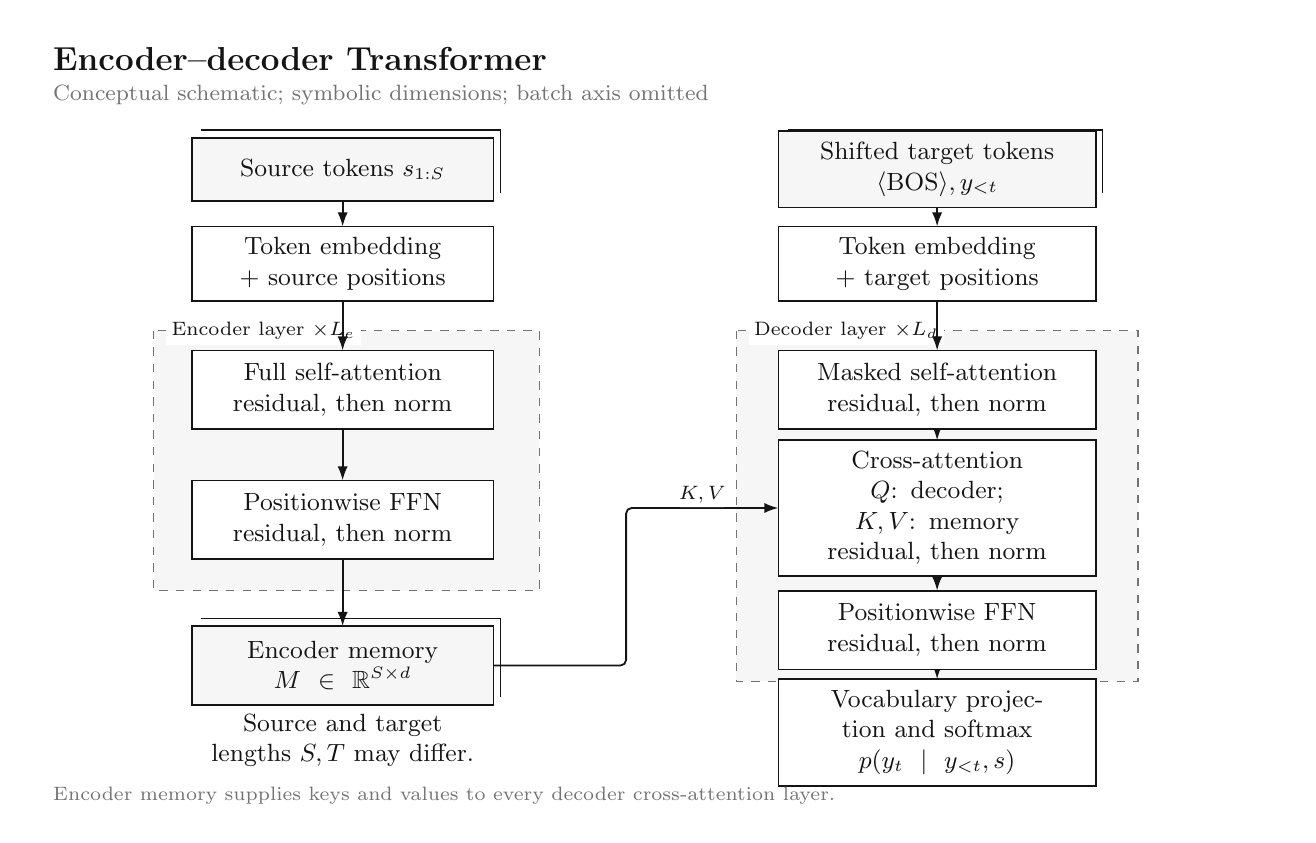
\begin{tikzpicture}[x=1cm,y=-1cm,font=\rmfamily,text=ink]

\path[use as bounding box] (0,0) rectangle (16,10);
\node[anchor=west,font=\large\bfseries] at (.2,.4) {Encoder--decoder Transformer};
\node[anchor=west,font=\footnotesize,text=soft] at (.2,.85) {Conceptual schematic; symbolic dimensions; batch axis omitted};
\begin{pgfonlayer}{background}
\draw[groupbox] (1.6,3.85) rectangle (6.5,7.15);
\node[anchor=west,font=\scriptsize,fill=white,inner sep=2pt] at (1.75,3.85) {Encoder layer $\times L_e$};
\draw[groupbox] (9.0,3.85) rectangle (14.1,8.3);
\node[anchor=west,font=\scriptsize,fill=white,inner sep=2pt] at (9.15,3.85) {Decoder layer $\times L_d$};
\end{pgfonlayer}
\node[box,fill=wash,minimum width=3.8cm,minimum height=0.8cm,text width=3.55cm] (src) at (4,1.8) {Source tokens $s_{1:S}$};
\draw[ink,line width=.4pt] (2.2,1.2999999999999998) -- (6.0,1.2999999999999998) -- (6.0,2.1);
\node[box,minimum width=3.8cm,minimum height=0.9cm,text width=3.55cm] (se) at (4,3) {Token embedding\\$+$ source positions};
\node[box,minimum width=3.8cm,minimum height=1.0cm,text width=3.55cm] (sa) at (4,4.6) {Full self-attention\\residual, then norm};
\node[box,minimum width=3.8cm,minimum height=1.0cm,text width=3.55cm] (sf) at (4,6.25) {Positionwise FFN\\residual, then norm};
\node[box,fill=wash,minimum width=3.8cm,minimum height=1.0cm,text width=3.55cm] (mem) at (4,8.1) {Encoder memory\\$M\in\mathbb{R}^{S\times d}$};
\draw[ink,line width=.4pt] (2.2,7.5) -- (6.0,7.5) -- (6.0,8.5);
\node[box,fill=wash,minimum width=4.0cm,minimum height=0.8cm,text width=3.75cm] (tgt) at (11.55,1.8) {Shifted target tokens\\$\langle\mathrm{BOS}\rangle,y_{<t}$};
\draw[ink,line width=.4pt] (9.65,1.2999999999999998) -- (13.65,1.2999999999999998) -- (13.65,2.1);
\node[box,minimum width=4.0cm,minimum height=0.9cm,text width=3.75cm] (te) at (11.55,3) {Token embedding\\$+$ target positions};
\node[box,minimum width=4.0cm,minimum height=1.0cm,text width=3.75cm] (ta) at (11.55,4.6) {Masked self-attention\\residual, then norm};
\node[box,minimum width=4.0cm,minimum height=1.15cm,text width=3.75cm] (cross) at (11.55,6.1) {Cross-attention\\$Q$: decoder; $K,V$: memory\\residual, then norm};
\node[box,minimum width=4.0cm,minimum height=1.0cm,text width=3.75cm] (tf) at (11.55,7.65) {Positionwise FFN\\residual, then norm};
\node[box,minimum width=4.0cm,minimum height=0.85cm,text width=3.75cm] (out) at (11.55,8.95) {Vocabulary projection and softmax\\$p(y_t\mid y_{<t},s)$};
\node[align=center,inner sep=0pt,outer sep=0pt,font=\small,minimum width=5.5cm,minimum height=0.5cm,text width=5.25cm] (note11) at (4,9.05) {Source and target lengths $S,T$ may differ.};
\begin{pgfonlayer}{background}
\draw[flow] (src.south) -- (se.north);
\draw[flow] (se.south) -- (sa.north);
\draw[flow] (sa.south) -- (sf.north);
\draw[flow] (sf.south) -- (mem.north);
\draw[flow] (tgt.south) -- (te.north);
\draw[flow] (te.south) -- (ta.north);
\draw[flow] (ta.south) -- (cross.north);
\draw[flow] (cross.south) -- (tf.north);
\draw[flow] (tf.south) -- (out.north);
\draw[flow] (mem.east) -- (7.6,8.1) -- (7.6,6.1) -- (cross.west) node[midway,above,fill=white,inner sep=1.5pt,font=\scriptsize] {$K,V$};
\end{pgfonlayer}
\node[anchor=west,align=left,font=\scriptsize,text=soft,text width=15.6cm] at (.2,9.75) {Encoder memory supplies keys and values to every decoder cross-attention layer.};
\end{tikzpicture}
\end{document}
